\documentclass{report}
\usepackage[utf8]{inputenc}
\usepackage{lib/report-template}
\usepackage[all]{background}
\usepackage{lipsum}

\SetBgContents{Preliminary version/2.0}% Set contents
\SetBgPosition{-0.5cm,-5.0cm}% Select location
\SetBgOpacity{1.0}% Select opacity
\SetBgAngle{90.0}% Select rotation of logo
\SetBgScale{2.0}% Select scale factor of logo


%Line spacing
\renewcommand{\baselinestretch}{1.5}

\title{projeto ATLAS}

\date{August 2019}


\begin{document}

\begin{titlepage}.
    \begin{tikzpicture}[remember picture,overlay]

% UTT Background under the title and info box
\coordinate [right=8mm, below=80mm] (uttbackground_anchor) at (current page.north west);
\node [name=uttsquare,anchor=north west] at (uttbackground_anchor){
%\includegraphics[width=19.4cm]{first-page-background.png}};
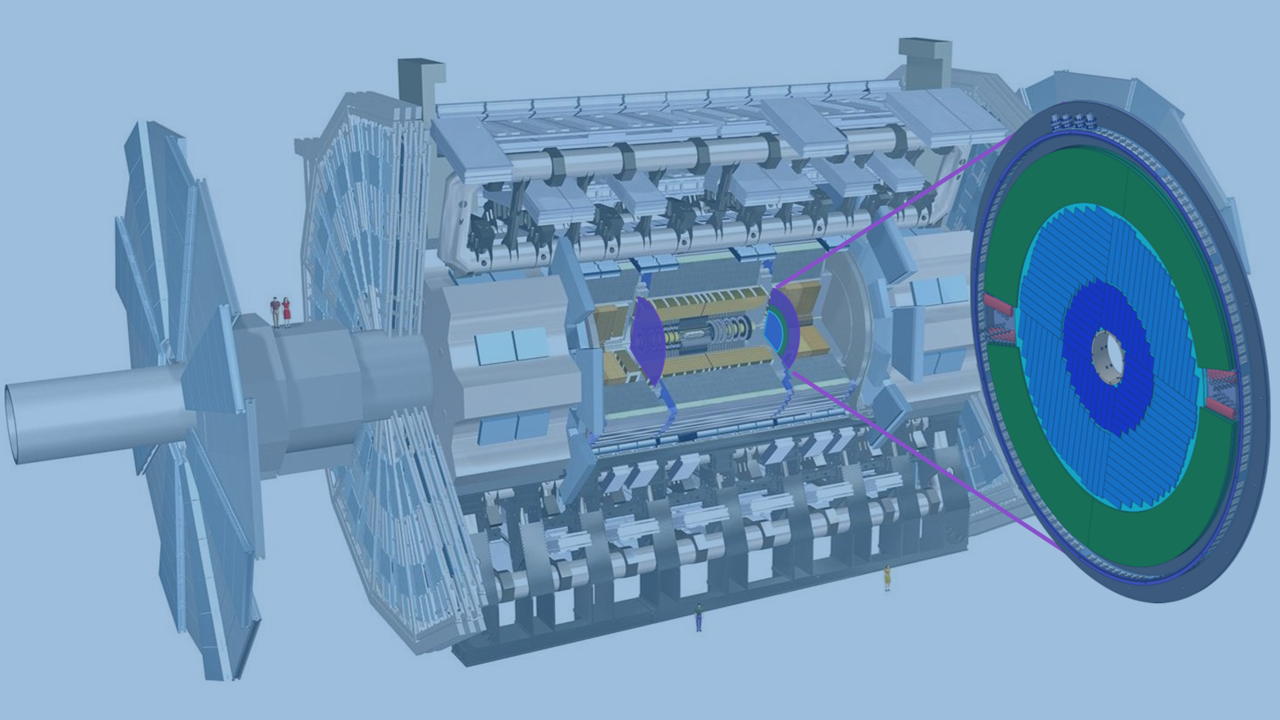
\includegraphics[width=19.4cm]{assets/ATLAS_BACKGROUND.png}};

\end{tikzpicture}

    % Margin to begin the text under the uttsquare
    \vspace{3.5cm}

    % Internship title
    
    \begin{textblock*}{15cm}(3cm,2cm)
        \begin{Huge}
            \begin{center}
                \makeatletter
                \noindent\textcolor{black}{UNIVERSIDADE DE SÃO PAULO \\ INSTITUTO DE FÍSICA}
                \makeatother
            \end{center}
        \end{Huge}
    \end{textblock*}
    
    % project tipe
    \begin{textblock*}{15cm}(2.5cm,5.5cm)
        \makeatletter
        \begin{LARGE}
            \begin{center}
                \color{black}
                {\it Projeto de pesquisa de pós-doutorado em física }\\
            \end{center}
         \end{LARGE}
     
    \end{textblock*}
    
    %TITLE
    \begin{textblock*}{15cm}(3cm,12cm)
        \begin{Huge}
            \begin{center}
                \makeatletter
                \noindent\textcolor{white}{Desenvolvimento de um detector de silício para a medida de trajetórias e tempo no experimento ATLAS-LHC}
                \makeatother
            \end{center}
        \end{Huge}
    \end{textblock*}

    % Author
    \begin{textblock*}{15cm}(2.5cm,20cm)
        \begin{LARGE}
        \begin{center}
            \color{black}
                \textbf{Autor :} Dr. Renato Aparecido Negrão de Oliveira \\ CERN \\ 
        \end{center}
            
        \end{LARGE}
        
    \end{textblock*}
    
    % FOOT NOTE
    \begin{textblock*}{15cm}(3cm,24cm)
        \makeatletter
        \begin{center}
            {\color{black}
                \textbf{SÃO PAULO, 2020} 
            }
        \end{center}
        \makeatother
    \end{textblock*}

\end{titlepage}

\begin{titlepage}.
    \begin{tikzpicture}[remember picture,overlay]

% UTT Background under the title and info box
\coordinate [right=8mm, below=80mm] (uttbackground_anchor) at (current page.north west);
\node [name=uttsquare,anchor=north west] at (uttbackground_anchor){
%\includegraphics[width=19.4cm]{first-page-background.png}};
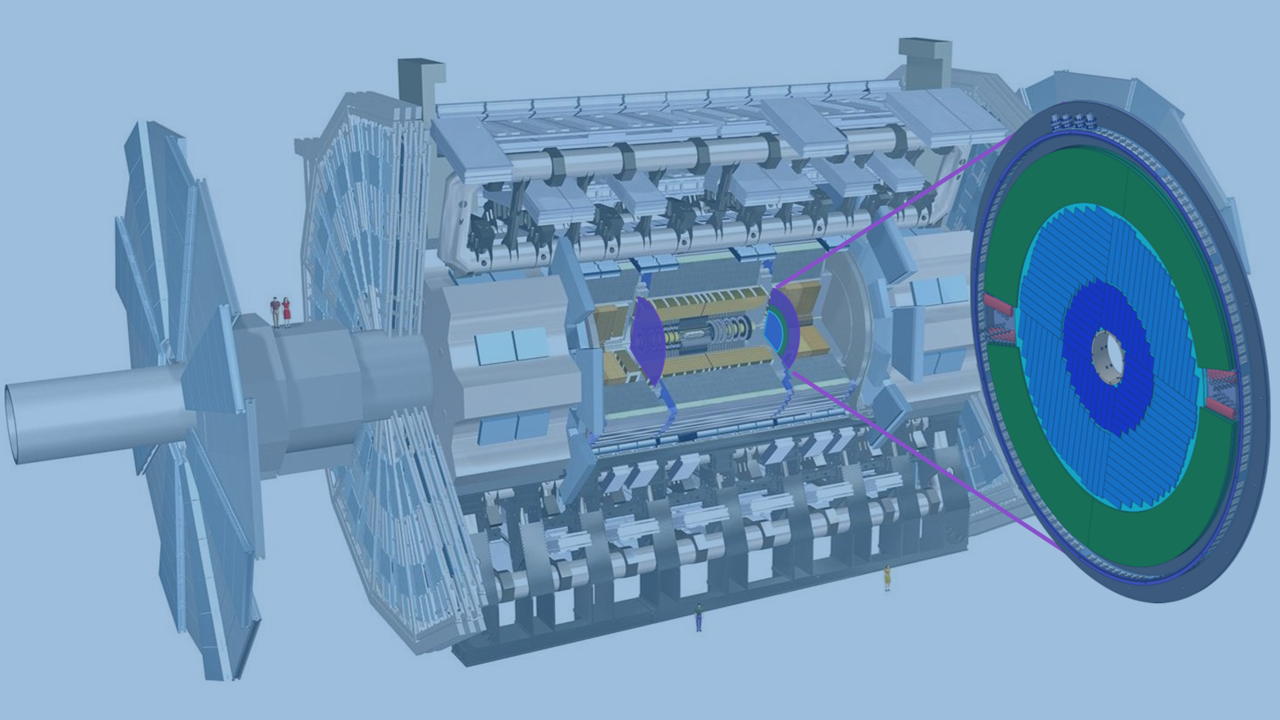
\includegraphics[width=19.4cm]{assets/ATLAS_BACKGROUND.png}};

\end{tikzpicture}

    % Margin to begin the text under the uttsquare
    \vspace{3.5cm}

    
    % Authhor
    \begin{textblock*}{15cm}(3cm,2.cm)
        \makeatletter
        \begin{huge}
            \begin{center}
                \color{black}
                 Renato Aparecido Negrão de Oliveira\\ 
            \end{center}
         \end{huge}
     
    \end{textblock*}
    
    %TITLE
    \begin{textblock*}{15cm}(3cm,12cm)
        \begin{Huge}
            \begin{center}
                \makeatletter
                \noindent\textcolor{white}{Desenvolvimento de um detector de silício para a medida de trajetórias e tempo no experimento ATLAS-LHC}
                \makeatother
            \end{center}
        \end{Huge}
    \end{textblock*}

    % Info box
    \begin{textblock*}{15cm}(2.5cm,20cm)
        \makeatletter
        \begin{LARGE}
            \setcellgapes{4pt}
            \makegapedcells
            {\color{black}\begin{tabularx}{15cm}{XX}
                \textbf{Supervisor :} Dr. Marco Aurélio Lisboa Leite (IFUSP)\\ 
                %\textbf{Supervisor :} Dr. Marcelo Gameiro Munhoz (IFUSP)
            \end{tabularx}}
        \end{LARGE}
        \makeatother
    \end{textblock*}
    
    % FOOT NOTE
    \begin{textblock*}{15cm}(3cm,24cm)
        \makeatletter
        \begin{center}
            {\color{black}
                \textbf{SÃO, PAULO 2020} 
            }
        \end{center}
        \makeatother
    \end{textblock*}

\end{titlepage}


\chapter*{Resumo}

%A necessidade de desenvolver detectores semicondutores rápidos para a medida de trajetória de partículas carregadas no {\it Large Hadron Collider} (LHC) tem aumentado no decorrer da última década em resposta ao aumento da luminosidade do feixe produzido no LHC.

Com o crescente aumento da luminosidade do feixe produzido no LHC, que será três vezes maior após o seu upgrade \cite{tdr}, inúmeros desafios experimentais são colocados, dentre eles está a identificação do grande número de colisões que ocorrem durante o cruzamento do feixe no LHC. A vista disso, uma forma de abordar os efeitos do empilhamento de colisões, e mitigar esse problema, é através do uso de técnicas de medida de tempo com alta precisão para distinguir as colisões que não podem ser separadas espacialmente. 

Para solucionar esse problema, um novo sistema de detecção será construído - denominado {\it High Granularity Timing Detector} (HGTD) - para a fase II do experimento ATLAS, o qual é baseado em sensores semicondutores de silício e cuja tecnologia empregada permite operá-los em um regime de baixo ganho de carga ({\it Low Gain Avalanche Detector} - LGAD). Esse detector será instalado na região frontal do experimento, cobrindo o intervalo em pseudo-rapidez de $2.4< |\eta| <4.0$, e permitirá medir intervalos de tempo da ordem de 20-30 pico segundos.

%Por conseguinte, a medida precisa do tempo irá melhorar a reconstrução do vértice da colisão, tendo em vista que diminui as incertezas na associação das trajetórias ao vértice onde foram originadas, possibilitando o aumento significativo do desempenho, e permitindo reconstruir jatos de partículas com grande precisão. A melhoria na capacidade de reconstrução de jatos - que será obtida com o HGTD - aumentará a sensibilidade do experimento permitindo explorar observáveis antes não explorados devido aos limites experimentais.

A vista disso, neste projeto de pós-doutorado é proposto o desenvolvimento de atividades de pesquisa junto ao grupo de pesquisa HEPIC da Universidade de São Paulo em colaboração com o experimento ATLAS do CERN. O trabalho será focado na pesquisa e desenvolvimento dos sensores semicondutores do tipo LGAD - recentemente desenvolvidos visando aplicações que requerem grande tolerância à altos níveis de radiação ionizante \cite{JIN_LGAD,NIMA_LGAD} - com o objetivo de optimizar sua capacidade para utilização no ATLAS. %A consolidação desse tipo de sensores oferece uma grande oportunidade em termos de pesquisa e desenvolvimento na área de sensores semicondutores, com aplicações em diversas áreas da física e tecnologia em geral.


\chapter*{Abstract}

%The development of fast response semiconductor sensor for particle tracking at LHC has increased in the past decade in response to the high luminosity expected for the upgraded Large Hadron Collider (LHC).

The significant increase of pile-up interactions by a factor three \cite{tdr} is one of the main experimental challenges for the High Luminosity LHC physics program, and a new way to mitigate the effects of pile-up is to use high-precision timing information to distinguish between collisions occurring close in space but well-separated in time.

To address this experimental challenge, a High-Granularity Timing Detector (HGTD), based on low gain avalanche detector technology is proposed for the ATLAS Phase-II upgrade. The detector will be installed at the forward region, covering the pseudorapidity range between $2.4< |\eta| <4.0$, and allowing the measurement of the time interval of the order of picoseconds.

%The high-precision timing information will greatly improve the track-to-vertex association, leading to a significant increase in performance allowing for a high-precision reconstruction of particle jets. These improvements in jet reconstruction performance will translate into important sensitivity gains and enhance the reach of the ATLAS physics program.

In this project, it is proposed to be performed activities on research and development at São Paulo University in collaboration with ATLAS experiment. The research will be focused on the development of the LGDA sensors - recently developed to operate at higher levels of radiation dose - to optimize the device capabilities to operate in the ATLAS experiment. The consolidation of this type of sensors offers a unique opportunity for research and development regarding the semiconductor sensors, with a great spin-off for other areas of physics and general technology.

\tableofcontents

\chapter{Introdução}

% 4 - IMPORTANCIA PARA O ATLAS UPGRADE
Para o experimento ATLAS, o desafio experimental é reconstruir partículas na região de rapidez frontal, produzidas na interação inicial de modo a associá-las corretamente com o vértice onde foram originadas, em um regime de altas taxas de colisão. Para solucionar esse desafio, um novo sistema de detecção frontal, denominado HGTD ({\it High Granularity Timing Detector}), está sendo desenvolvido - com base nos sensores LGAD - para fornecer uma medida precisa de tempo, com o objetivo de diminuir os efeitos do {\it pile-up} dos eventos. 

De modo geral, a capacidade de associar as trajetórias ao vértice primário depende da precisão na determinação do parâmetro de impacto longitudinal. Enquanto que para trajetórias centrais com pseudo-rapidez no intervalo $\eta<1.5$, o parâmetro de impacto longitudinal é pequeno e determinado com grande precisão, para trajetórias frontais com $\eta>2.5$ o parâmetro de impacto cresce rapidamente atingindo valores da ordem de milímetros \cite{tdr}. Esse é um comportamento perfeitamente explicado pelo fato delas tornarem se mais colineares com a linha do feixe, o que associado à segmentação do detector dificulta a extrapolação das trajetórias para a posição do vértice da colisão, resultando em grandes valores obtidos para o parâmetro de impacto longitudinal.

Desse modo, devido à baixa resolução presente na medida da proximidade longitudinal ao vértice primário, trajetórias frontais são mais difíceis de associar de forma não ambígua com o vértice do evento. Devido a isso, e para preservar a excelente resolução obtida para as trajetórias centrais, com a construção e utilização do HGTD o experimento ATLAS será capaz de associar com grande precisão trajetórias frontais ao vértice da colisão para eventos que acontecem muito próximos no espaço, entretanto em instante de tempo distintos. Utilizando a informação do tempo em que as colisões acontecem - fornecida pelo HGTD - será possível identificar quais trajetórias frontais pertencem a um determinado vértice rejeitando trajetórias originadas em outras interações espacialmente próximas ao vértice em questão. 

Por conseguinte, com o aumento significativo da eficiência na medida de partículas frontais através do uso do HGTD será possível medir com precisão a luminosidade do feixe, que é uma medida crítica para a determinação da seção de choque de produção de partículas em diversas analises físicas, além de  permitir a reconstrução de jatos de partículas com grande precisão. A melhoria na capacidade de reconstrução de jatos - que será obtida com o HGTD - aumentará a sensibilidade do experimento, permitindo explorar observáveis antes não explorados devido aos limites experimentais.

%4.1 porque esoolheram o lgad
\begin{figure} 
    \centering
    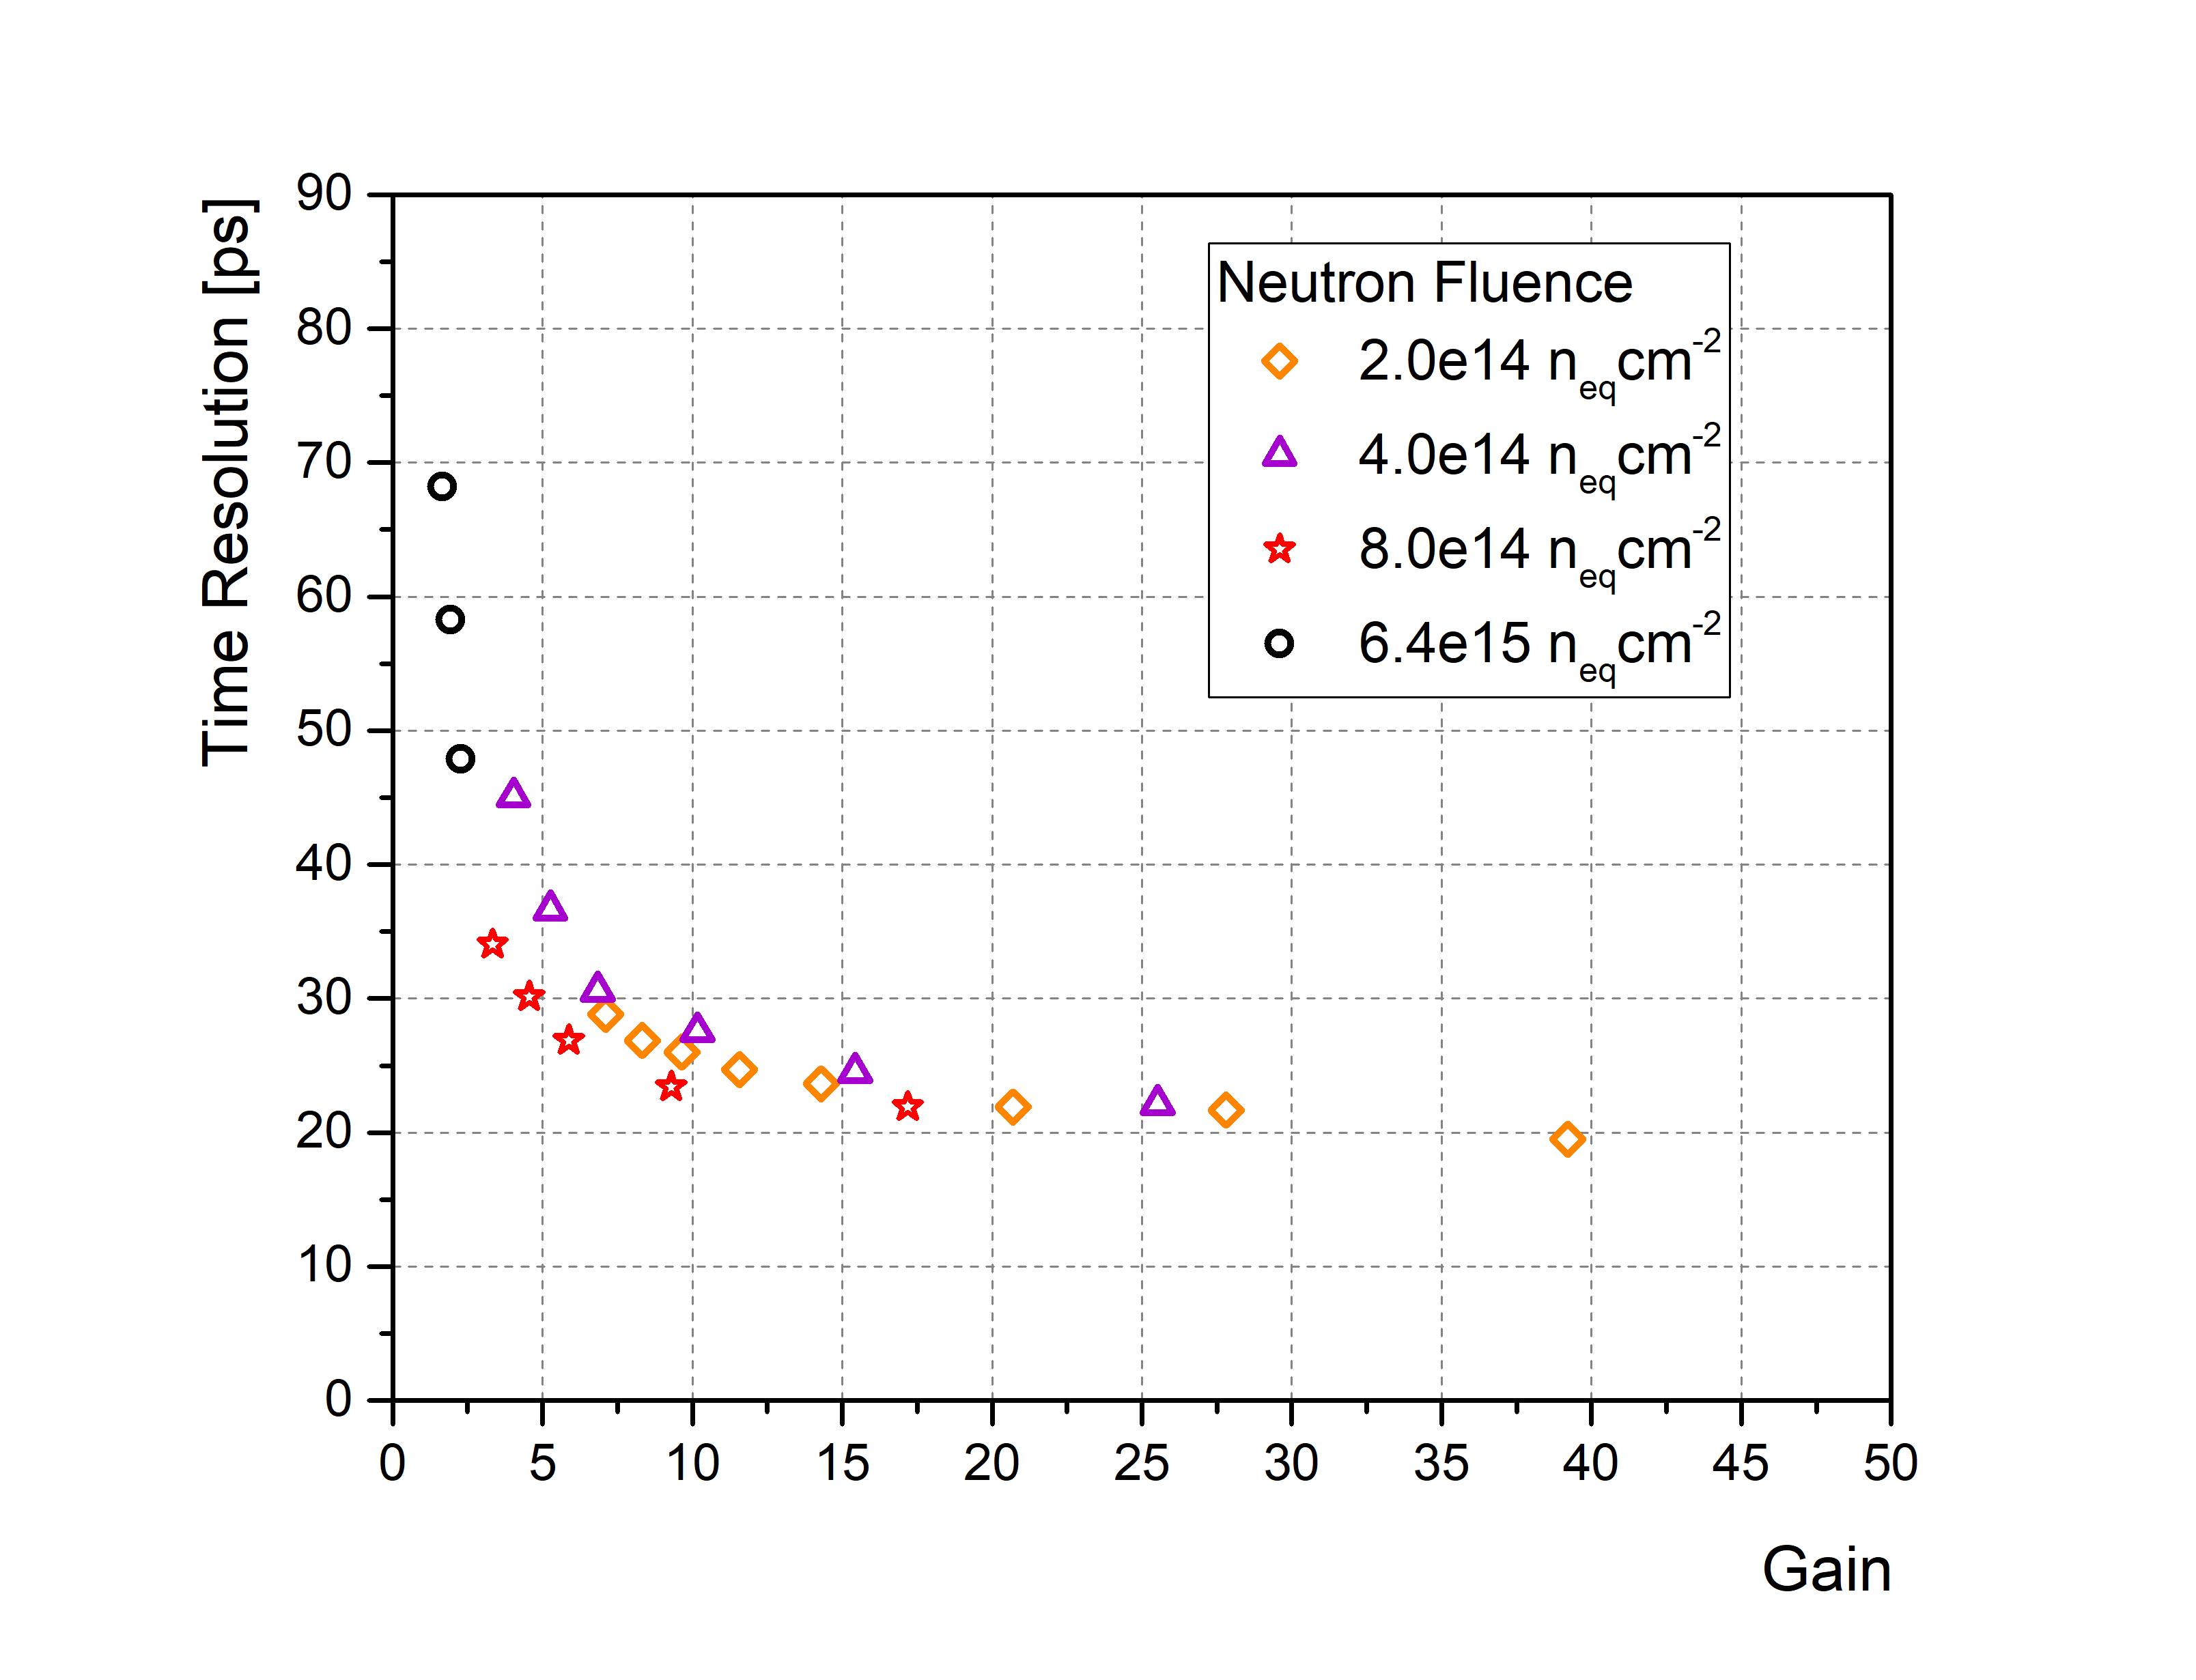
\includegraphics[width=12.0cm]{assets/timeresolution_vs_gain.png}
    \caption{ Gráfico mostrando a resolução temporal em função do ganho do LGAD. Dados retirados da referência \cite{tdr}.}
    \label{timeresolution}
\end{figure}

Neste ponto cabe destacar que os sensores LGAD foram adotados como base tecnológica para a construção do HGTD por apresentarem excelentes características com respeito ao compromisso entre ganho e resolução temporal. A Fig. \ref{timeresolution} mostra quatro conjuntos de dados medidos - utilizando os primeiros protótipos do sensor irradiados em  diferentes valores de fluência de nêutrons - onde é possível observar a dependência da resolução em tempo em função de seu ganho. De acordo com os dados, eles demonstram que é possível atingir resolução em tempo menores que 30ps com valores moderados de ganho.    
Por conseguinte, como ilustra a Fig. \ref{hgtd}, o HGTD foi concebido para ser instalado na região frontal do experimento, em ambos os lados a uma distancia de $3.5m$ do ponto de interação do feixe, região a qual está localizada após o volume do ATLAS {\it Inner Tracker} (ITk) \cite{tdr}. 

\begin{figure} 
    \centering
    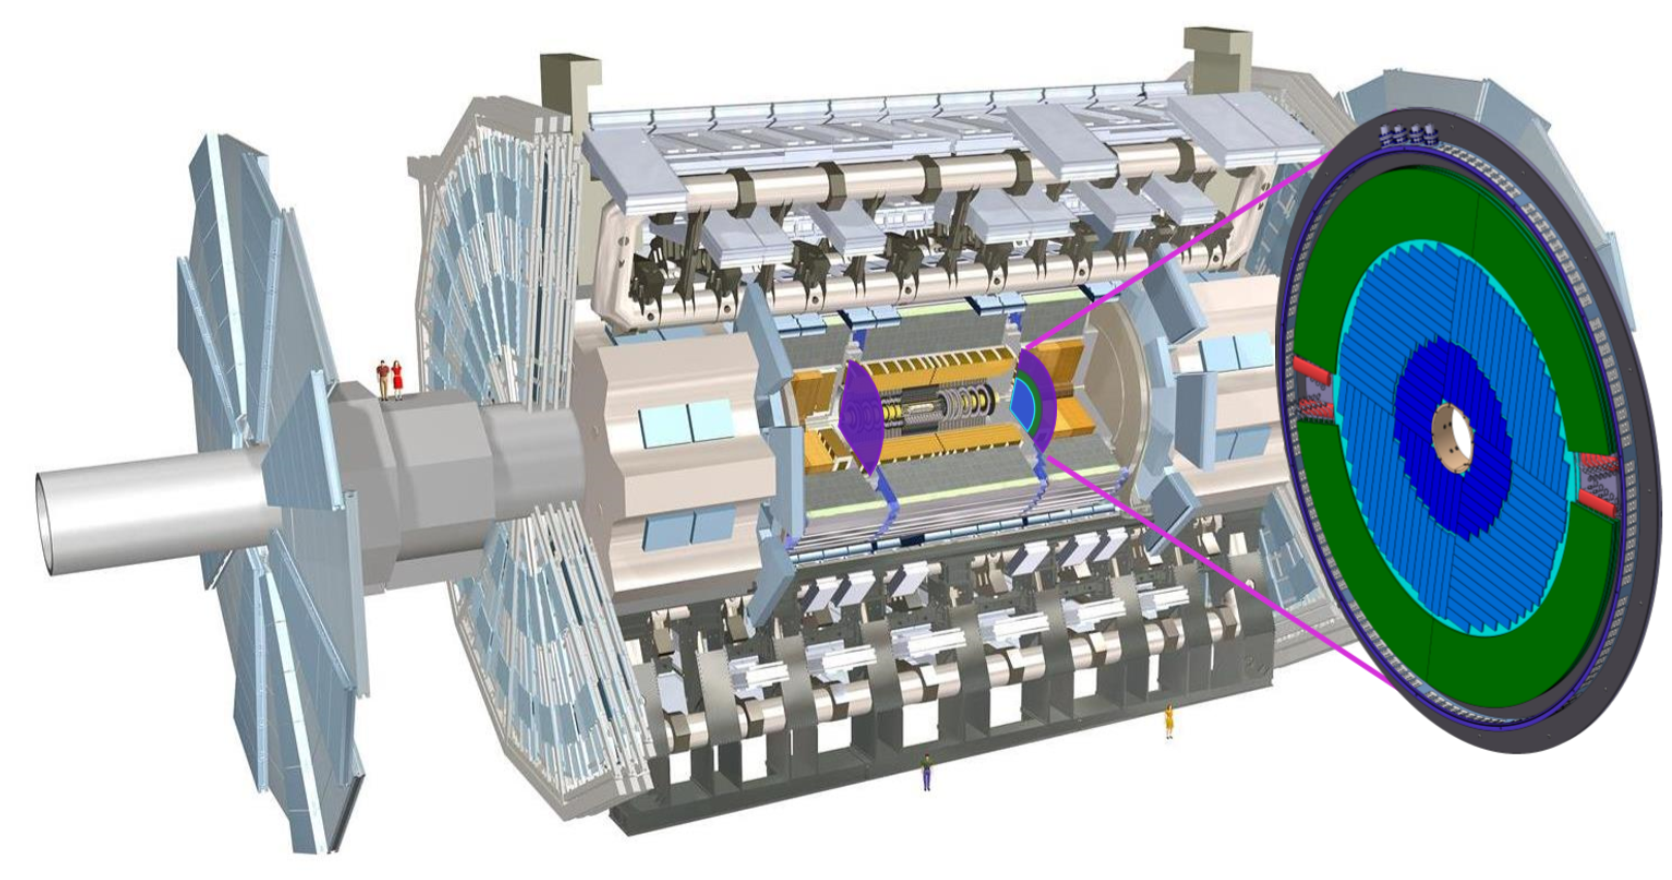
\includegraphics[width=15.0cm]{assets/ATLAS_HGTD.png}
    \caption{ Figura mostrando no detalhe mostra a posição onde o HGTD será instalado. Figura também mostra o experimento ATLAS e os seus vários sistemas.}
    \label{hgtd}
\end{figure}

% 1 - IMPORTANCIA DO PROJETO
Detectores semicondutores de resposta rápida do tipo LGAD ({\it Low Gain Avalanche Detector}) é uma tecnologia introduzida recentemente no escopo do desenvolvimento de sensores semicondutores \cite{JIN_LGAD,NIMA_LGAD}, cuja capacidade de produzir sinais em intervalos de tempo muito curtos possibilita a medida de eventos produzidos em colisões p-p nos experimentos de física de altas energias em intervalos de tempo da ordem de pico segundos. 

Além da resposta rápida à incidência de radiação, esse tipo de sensor possui ganho intrínseco devido ao perfil de dopagem empregado no material semicondutor, o que torna possível amplificar o sinal produzido e dessa forma operá-lo em modo de avalanche de carga \cite{JIN_LGAD,NIMA_LGAD}. Essas características demonstram a complexidade e a importância dessa tecnologia para o desenvolvimento da próxima geração de sensores semicondutores para aplicações que requerem altas taxas de contagem.

% 2 - PROPOSTA DO PROJETO
Os primeiros sensores baseados em LGAD foram desenvolvidos no Centro Nacional de Microeletrônica (CNM) em Barcelona e posteriormente pela colaboração RD50-CERN \cite{tdr,JIN_LGAD,NIMA_LGAD}, a qual é uma colaboração localizada no CERN que visa desenvolver detectores semicondutores para aplicações com feixes de alta intensidade.% Além disso, o RD50 promove o surgimento de novas aplicações e inovações através do desenvolvimento de ferramentas e da consolidação do conhecimento e dos fenômenos físicos relacionados com sensores semicondutores. 

Em maiores detalhes, LGAD são sensores semicondutores planos com ganho intrínseco como ilustra a Fig. \ref{lgad}. O ganho do sensor é determinado pela quantidade de dopante implantado na matriz de silício formando a camada de multiplicação. Como mostra a Fig. \ref{lgad}, sua arquitetura é composta de uma camada de material semicondutor do tipo n sobre uma camada do tipo p, com a adição de uma camada altamente dopada do tipo p localizada entre a junção n-p, cuja função é criar um alto campo elétrico responsável por produzir a avalanche das cargas e amplificar o sinal elétrico. Dessa forma, quando uma partícula atravessa a região sensível do detector  elétrons e lacunas são criados produzindo uma corrente inicial. Os elétrons ao atingirem a região de amplificação produzem novos pares elétron lacuna sendo desse modo multiplicados em um processo de avalanche. Essa corrente, de 10 a 30 vezes maior do que a produzida em um diodo padrão, é o principal mecanismo responsável pela excelente resolução em tempo desses sensores. 

\begin{figure}
    \centering
    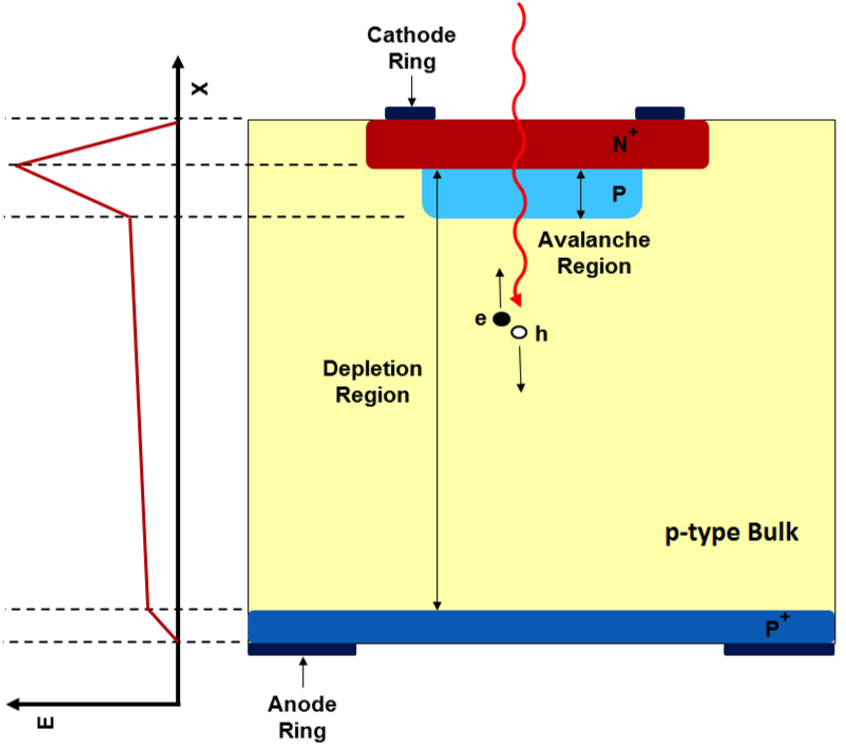
\includegraphics[width=7.0cm]{assets/lgad.png}
    \caption{Figura mostrando a estrutura esquemática de um sensor LGAD.}
    \label{lgad}
\end{figure}

% 3 - BREVE PROPOSTA DO PROJETO
À vista disso, um dos propósitos deste projeto é desenvolver técnicas e metodologias necessárias para a caracterização física de sensores semicondutores do tipo LGAD. Neste escopo a colaboração com o experimento ATLAS no CERN será fundamental pois irá servir de ponte para a troca de conhecimento e experiência permitindo introduzir esse tipo de tecnologia no IFUSP.

%-------------------- 4.1 colocar algo mais com respeito ao btagging e reconstrucao de jatos 
% para a realizacao deste detector sera empregado sensore LGAD....
% 5 - DETALHE DA TIMELINE OBJETIVO
Com isso em mente, em maiores detalhes, neste projeto de pesquisa é proposto o desenvolvimento de atividades focadas na pesquisa e desenvolvimento dos sensores semicondutores do tipo LGAD com o objetivo de optimizar sua característica para utilização no HGTD do experimento ATLAS. A consolidação desse tipo de sensores oferece uma grande desafio em termos de pesquisa e desenvolvimento na área de sensores semicondutores, com potencial de aplicação em diversas áreas da física e tecnologia em geral. 

O projeto será composto de várias etapas. Inicialmente pretende-se consolidar as técnicas necessárias para a caracterização dos sensores. Neste processo o pesquisador responsável e colaboradores irão estabelecer o métodos experimentais para a caracterização das propriedades físicas dos sensores. Nesta estágio, o pesquisador será responsável por montar e certificar os arranjos experimentais, desenhar e construir as parte necessárias para os mesmos, além de automatizar o processo de tomada de dados. Por fim, a comparação direta com resultados obtidos em outros centros de pesquisa dentro da colaboração ATLAS será feita para garantir a qualidade dos resultados obtidos e acelerar a consolidação dessa etapa.  
Uma vez que a primeira etapa seja concluída, sensores LGAD serão irradiados no reator multipropósito localizado no IPEN, e em seguida serão caracterizados no setup previamente estabelecido com o objetivo de estudar o comportamento do ganho e resolução em tempo do sensor em função da fluência das partículas atravessando o volume sensível do detector. Essa etapa é fundamental para compreender os mecanismos associados à física do dano radioativo em sensores semicondutores e por conseguinte propor melhorias para a próxima geração de sensores. 
Neste ponto cabe destacar que as metodologias e técnicas desenvolvidas na pesquisa de novas tecnologias que aumentem a resistência dos sensores ao dano radioativo, são extremamente importantes do ponto de vista científico e tecnológico uma vez que possibilitarão a geração de conhecimento com respeito aos efeitos físicos da radiação em materiais semicondutores dopados ainda não bem conhecidos \cite{tdr,JIN_LGAD,NIMA_LGAD}. %Neste âmbito os processos e métodos desenvolvidos na pesquisa poderão ser convertidos na produção de patentes. 
Em seguida com base nos dados coletados nesta fase de teste dos protótipos, será possível estabelecer com grande precisão as especificações que melhor atendem as necessidades do experimento ATLAS. 

Uma vez optimizados, a solução definida será produzida em larga escala, e neste ponto o grupo fará parte do esforço em conjunto com o experimento ATLAS para qualificar os sensores que serão empregados na construção do HGTD. Essa etapa é fundamental para o exercício dos métodos desenvolvidos nas etapas anteriores bem como para a consolidação da importância do grupo de pesquisa HEPIC na esfera da colaboração ATLAS.

%-- estará contato com o Laboratório de novos materiais semicondutores da USP
%Em uma segunda frente de pesquisa, no âmbito nacional, através da coloração com o Laboratório de Sistemas Integráveis (LSI) da Escola Politécnica da USP - colaboração essa previamente estabelecida em projetos anteriores executados com o HEPIC \cite{ALICEUP,ref1} - será possível, através da transferência de know how, produzir sensores LGAD com o objetivo de melhorar a sua tecnologia e explorar o seu grande potencial para aplicações em outras áreas da ciência. Nessa frente de pesquisa, o pesquisador responsável irá gerenciar as tecnologias e recursos técnicos disponíveis no LSI com o objetivo de obter os melhores resultados para a produção do LGAD.  

% 6 - APLICACOES PARA A INDUSTRIA
%Ainda no ambito nacional, pretende se fazer um esforço ...
% 7 - PONTOS POSITIVOS DO GRUPO
Por fim, é importante destacar que a implantação dessa linha de pesquisa no HEPIC será de extrema importância para projetos futuros envolvendo sensores semicondutores. Atualmente o grupo conta com excelentes ferramentas na areá de instrumentação para física nuclear e de partículas reconhecida internacionalmente, e adquirida por meio da execução de projetos em colaborações internacionais, como por exemplo o chip SAMPA focada na tecnologia de detectores gasosos \cite{ref1}. Isso somado à experiência do pesquisador responsável adquirida na execução de pesquisa e desenvolvimento no âmbito do projeto de upgrade do TPC do ALICE \cite{tpcNIM,discharge_paper}, tornará possível a transferência total de tecnologia relacionada com sensores semicondutores de alta performance para o HEPIC, bem como a geração de novas tecnologias e aplicações que poderão estabelecer o grupo como um protagonista internacional.
% Conteúdo do capitulo 
% 1- Desenvolver e caracterizar sensores LGAD para o upgrade do ATLAS
%2- Estudar experimentalmente os processos físicos relacionados com a amplificação da carga
%3- Melhorar os sensor por intermédio de simulações comparando com dados experimentais
%4- Desenvolvimento de um sistema de aquisição
%5- perspectivas de outros trabalhos
\chapter{Objetivos do projeto}

% 1- Desenvolver e caracterizar sensores LGAD para o upgrade do ATLAS
O objetivo deste projeto é caracterizar e desenvolver sensores semicondutores do tipo LGAD para o upgrade do experimento ATLAS, bem como para outras aplicações no âmbito do Instituto de Física da USP. O trabalho será dividido em fases as quais visam em um primeiro momento consolidar o {\it know how} sobre essa tecnologia no HEPIC, e em um segundo momento, com as competências consolidadas, contribuir para a melhoria do sensor e suas aplicações em diversas áreas da ciência, bem como para o ATLAS.

Como exposto anteriormente, no contexto da colaboração ATLAS, o pesquisador responsável participará ativamente na qualificação dos sensores e na consolidação de suas especificações. Em seguida, uma vez definidos os sensores, os mesmos serão produzidos em larga escala, e neste ponto o grupo fará parte do esforço em conjunto com o experimento ATLAS para qualificar os LGAD que serão empregados na construção do HGTD. Esse trabalho será fundamental para o exercício dos métodos a serem desenvolvidos.% bem como para a c da importância do grupo de pesquisa HEPIC na esfera da colaboração ATLAS.

%2- Estudar experimentalmente os processos físicos relacionados com a amplificação da carga
Em seguida, com a implantação das diversas metodologias experimentais para a caracterização dos sensores semicondutores será possível estudar em grande detalhe os processos físicos relacionados com a amplificação de carga e a produção de sinal no material semicondutor, visando compreender e melhorar os processos de fabricação baseando-se no aumento do ganho, resolução temporal e estabilidade elétrica dos sensores durante sua operação em ambiente com alta radiação \cite{tdr}. 
Como resultado espera-se produzir novas gerações de sensores os quais poderão ser utilizados não apenas para a detecção de partículas carregadas, mas como detector de raios-X. Devido às excelentes características dos detectores do tipo LGAD, as quais incluem sua alta eficiência quântica para uma grande faixa de comprimentos de onda e a possibilidade de construir detectores com alta granularidade, aplicações em diversos ramos envolvendo a detecção de raios-X, tais como luz síncrotron, tornam-se muito atrativas e de fácil implantação uma vez estabelecida essa tecnologia. Essa também é uma das propostas do projeto para longo prazo.

%3- Melhorar os sensor por intermédio de simulações comparando com dados experimentais
Outro aspecto importante que também será trabalhado neste projeto é o estudo de melhorias na geometria do LGAD por intermédio de simulações e modelos computacionais, e a comparação direta com dados experimentais medidos em laboratório para a validação do modelo. Esse trabalho será fundamental para possibilitar a melhoria do sensor, além de produzir um modelo validado capaz de fazer predições para o caso de novos designs de sensores semicondutores. 

%4- Desenvolvimento de um sistema de aquisição
Além do desenvolvimento dos sensores LGAD, um outro objetivo deste projeto será o de integrá-lo a um sistema de aquisição de dados, o que tornará possível a reconstrução de eventos. Como resultado espera-se desenvolver todas as competência e habilidades presentes nos diversos componentes que compõem o sistema de aquisição, desde os aspectos físicos relacionados com a produção do sinal até o tratamento dos dados e imagens produzidas.

%5- perspectivas de outros trabalhos
%Por fim, o desenvolvimento de algorítimos para a reconstrução dos dados do experimento ATLAS utilizando o HGTD em conjunto com o ITk não serão inclusos de início como objetivos neste projeto, no entanto tendo em vista a importância deste componente para o desenvolvimento do sistema de detecção e aquisição o mesmo poderá, como uma perspectiva futura, ser trabalhado mais adiante no projeto. %dependendo da quantidade de recursos disponíveis para serem realocados para essa atividade.  

% Este projeto tem como objetivo estrategico preparar o terreno para projetos futuros no campo de semicondutores e para a continuacao com projetos tematicos.
\renewcommand{\cleardoublepage}{}
\renewcommand{\clearpage}{}
% Conteúdo do capitulo
%1 - Descrição do desafio experimental para o ATLAS
%2 - Desafio de estabelecer o setup experimental
%3 - Desafio de melhorar o sensor LGAD
%4 - Desafio de aplicar para a medida de raios-x
%5 Considerações finais
\chapter{Desafios científicos e tecnológicos}

% 1 - Descrição do desafio experimental para o ATLAS
Como descrito anteriormente no texto desta proposta, o desafio científico deste projeto é desenvolver um detector semicondutor - para a região de pseudo-rapidez frontal - capaz de melhorar a precisão da medida de luminosidade do feixe e a reconstrução de partículas no experimento ATLAS, para operar durante a fase de alta luminosidade do LHC ({\it High Luminosity LHC} (HL-LHC)) \cite{tdr}. 

Para superar esse desafio científico, este projeto irá trabalhar na pesquisa e desenvolvimento de um sistema de detecção frontal HGTD, cuja a técnica experimental é baseada na medida do tempo de voo das partículas com resolução capaz de medir intervalos de tempo da ordem de 20-30ps \cite{tdr}, tornando dessa forma possível associar as partículas ao seu vértice de produção para colisões próton-próton no HL-LHC. Para realizar a construção do HGTD, os sensores do tipo LGAD serão adotados como base tecnológica, tendo em vista que eles apresentam excelentes características com respeito ao compromisso entre ganho e resolução temporal. 

% FASE 1
%2 - Desafio de estabelecer o setup experimental
A fase inicial do projeto terá como foco o desenvolvimento da metodologia experimental necessária para a caracterização dos sensores LGAD. Isso será feito através da implantação de três técnicas no laboratório de análises no HEPIC, com o objetivo de caracterizar os sensores LGAD em termos de sua corrente de fuga, ganho, uniformidade e resolução temporal. Nos parágrafos seguintes são descritos os passos que serão dados neste projeto para superar os desafios tecnológicos postos ao pesquisador responsável por esta proposta. 

Inicialmente será construída uma bancada de testes capaz de medir a corrente de fuga e a capacitância em função da voltagem aplicada ao sensor. A Fig. \ref{setup1} mostra um diagrama esquemático do arranjo experimental previsto para ser comissionado para este propósito.

\begin{figure}
    \centering
    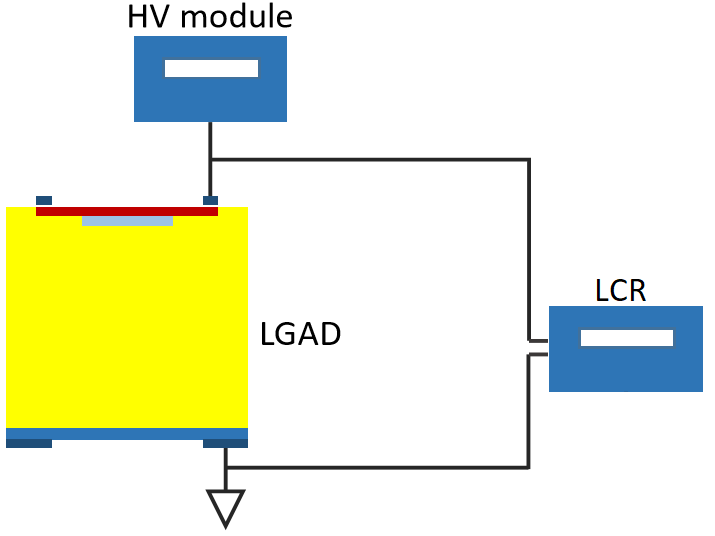
\includegraphics[width=10.0cm]{assets/iv_cv.png}
    \caption{Figura mostrando o diagrama para a medida de corrente e capacitância de um sensor LGAD.}
    \label{setup1}
\end{figure}

Em maiores detalhes, a montagem será composta por uma estação de prova onde os sensores serão acomodados durante os testes. Uma fonte de alta tensão com resolução para a medida de corrente será utilizada para aplicar a tensão e medir a corrente de fuga dos sensores - neste ponto cabe destacar que a utilização de pico amperímetros em conjunto com a fonte de tesão não é descartado. A medida da capacitância do LGAD será feita por intermédio de um Keysight LRC Analyser o qual permitirá medir a capacitância do sensor em função do bias aplicado. Por fim, todos esses equipamentos serão controlados por um programada de controle e aquisição dos dados o qual será produzido em ambiente LabView para monitorar as medidas e controlar sua qualidade.

Em seguida um setup dedicado será construído para medir o ganho dos sensores e a sua uniformidade. Nesta montagem será utilizado um laser vermelho de 660nm de pulso rápido - da ordem de pico segundos - o qual irá incidir na base do sensor produzindo elétrons de deriva devido à ionização do meio. Em seguida os elétrons serão coletados pelo campo elétrico presente na região de depleção do detector indo em direção à região de amplificação do dispositivo onde serão multiplicados. O sinal produzido neste processo será coletado no anodo e subsequentemente amplificado por intermédio de um amplificador externo sendo digitalizado em um osciloscópio. Finalmente, a carga coletada será medida através da integral da forma de onda fornecendo o valor do ganho do sensor. A uniformidade do sensor será medida com o mesmo princípio, por intermédio de uma varredura da posição de incidência do laser sobre a região sensível do sensor.

Por fim, para completar o conjunto de técnicas necessárias, a montagem de um sistema de medida precisa de tempo será feita para caracterizar os sensores em termos de sua resolução temporal. Para tanto serão necessários a utilização de uma fonte $\beta$ de $^{90}$Sr, um detector para atuar como trigger - o qual pode ser um detector Cherenkov de quartzo acoplado a um Silicon Photo Multiplier (SiPM) com resolução temporal de 10ps, ou outro sensor LGAD - e placas com eletrônica para acomodar o sensor e efetuar a leitura dos dados. Como mostra a Fig. \ref{setup2} neste arranjo o trigger será colocado atrás do LGAD, tornando possível medir apenas partículas com energia suficiente para atravessar o sensor. Neste sistema o trigger também será lido por um osciloscópio, e a resolução temporal será extraída da diferença entre a distribuição de tempo medida com o LGAD e o detector trigger.

\begin{figure}
    \centering
    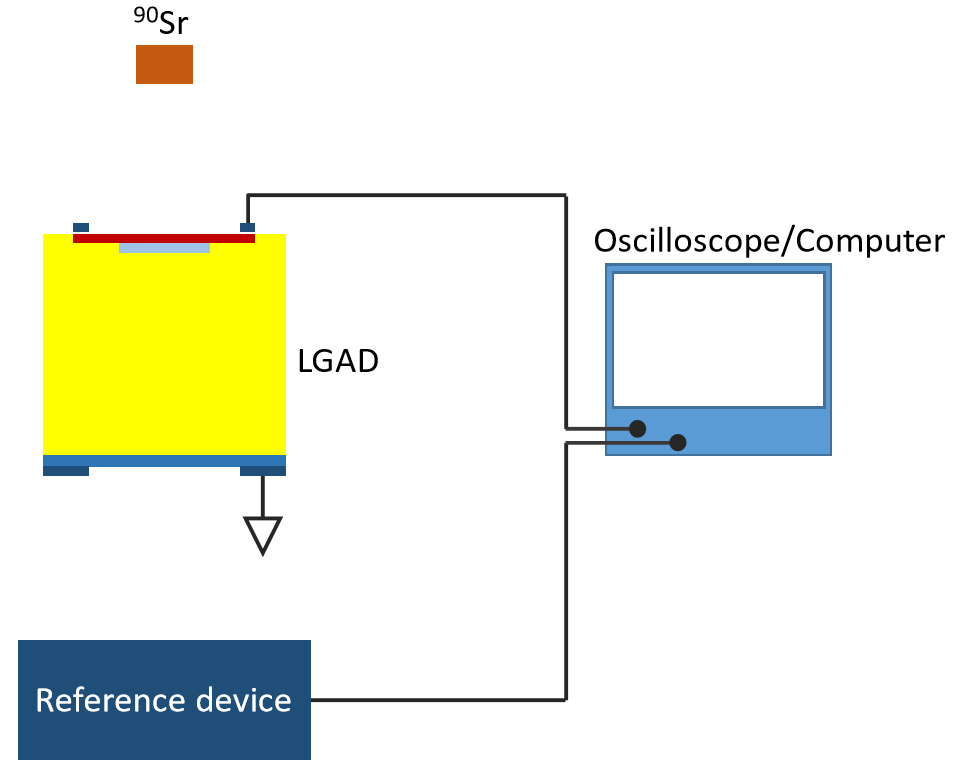
\includegraphics[width=10.0cm]{assets/time.png}
    \caption{Figura mostrando o diagrama para a medida da resolução temporal de um sensor LGAD.}
    \label{setup2}
\end{figure}

Com essas três técnicas estabelecidas será possível diagnosticar com precisão a qualidade dos sensores LGAD. Neste ponto, cabe ressaltar que o controle de temperatura é um componente importante para todas as técnicas de medida descritas anteriormente, e desse modo um controlador de temperatura será utilizado para estabilizar a temperatura do LGAD à -30$^{\circ}$ durante todas as medida que serão efetuadas, sendo essa a temperatura de operação nominal do HGTD \cite{tdr}.

À vista disso, cabe destacar que o grupo HEPIC possui competências adquiridas ao longo de anos de pesquisa dedicada a instrumentação que serão essenciais para o desenvolvimento deste projeto em sua fase inicial, tais como: design e confecção de placas eletrônicas para sensores, desenvolvimento de {\it Front End Electronics}, desenvolvimento de {\it Back End Electronics}, i.e firmware para aquisição de dados, e desenvolvimento de software para aquisição e análise de dados. Essas ferramentas aliadas à experiência do pesquisador responsável com o desenvolvimento de instrumentação científica \cite{tpcNIM,discharge_paper,THGEM} e com a colaboração com outros centros de pesquisa dentro da colaboração ATLAS será importante para estabelecer de forma rápida as técnicas descritas anteriormente, garantindo a qualidade dos resultados obtidos e o sucesso dos investimentos feitos para pesquisa e desenvolvimento desses sensores. 

% FASE 2 - PROTOTIPAGEM DO LGAD
%3 - Desafio de melhorar o sensor LGAD
Uma vez consolidada os experimentos descritos acima para a caracterização dos sensores LGAD, o passo seguinte será continuar com o desenvolvimento do dispositivo, e com base nos dados coletados buscar discutir e optimizar os parâmetros do sensor com o objetivo de produzir novas gerações de LGAD com melhores características em termos de ganho, resolução temporal, uniformidade e resistência à radiação. 

Como dito anteriormente, o programa de pesquisa proposto neste projeto será em grande parte baseado na interação com a colaboração ATLAS, de modo que teremos acesso aos recentes avanços obtidos no desenvolvimento do LGAD, tais como a identificação de vulnerabilidades presentes na geometria do sensor e a inativação do material dopante devido ao dano radioativo, os quais serão também tópicos para investigação neste projeto.

Em maiores detalhes, com relação à geometria do LGAD, no atual estágio de desenvolvimento foi possível identificar fragilidades em seu design relacionados com regiões suscetíveis à ocorrência de descargas elétricas presentes nas bordas do sensor, onde o campo elétrico aplicado é mais elevado. Essa vulnerabilidade afeta a estabilidade elétrica do sensor, e essa questão será atacada no desenvolvimento dos próximos protótipos através de melhorias em seu {\it layout} as quais diminuam o campo elétrico em regiões críticas do sensor \cite{tdr}.  
   
   % meio sem fluencia
Outro aspecto importante, o ganho em um detector LGAD é uma característica que depende diretamente do perfil da concentração de dopante presente na camada de multiplicação do sensor. Devido a presença dessa camada de amplificação o sensor torna-se mais complexo e mais suscetível à danos radioativos, levando em consideração que a inativação do dopante e a subsequente redução de sua concentração na camada de multiplicação pela incidência de radiação, provoca a redução do ganho e perdas na resolução em tempo. Para superar essa limitação tentativas preliminares demonstraram que a adição de outros materiais, tais como carbono, junto com o material dopante podem minimizar o impacto do dano radioativo tornando os sensores mais resistentes à radiação ionizante, entretanto com a contrapartida de diminuir a resolução em tempo \cite{tdr}. 

A vista disso, com a diminuição do ganho uma série de fatores surgem no escopo da pesquisa com o LGAD dentre eles o aumento da corrente consumida pelo dispositivo, o que por sua vez provoca o aumento na potência dissipada. Esse fator influencia o design de vários outros componentes que farão parte do detector para que seja possível dimensioná-los de forma adequada para comportar a carga de calor produzida pelo dispositivo. Estas questões  demonstram a grande importância de um estudo detalhado desses aspectos durante a fase de pesquisa e desenvolvimento do sensor. %Até o momento os requisitos para a potência dissipada do dispositivo LGAD estão em aberto e serão abordados na produção dos próximos protótipos.

O cronograma de excussão do projeto para o desenvolvimento do LGAD da colaboração ATLAS se estenderá até o início 2021, afim de validar as possíveis modificações adotadas com relação ao {\it layout}, materiais empregados e diversos componentes e processos que serão empregados na produção dos dispositivos. Isso é essencial para assegurar que pontos importantes em relação ao sensor e sua integração sejam revisados e verificados de modo a atender as especificações requeridas pelo experimento ATLAS.

Como fica claro, o design final do LGAD encontra-se em seu estágio inicial de desenvolvimento, e desse modo inúmeras oportunidades para contribuição intelectual estão em aberto para serem exploradas na próxima fase da pesquisa e desenvolvimento que está para ser iniciada. De forma objetiva, o cronograma do projeto prevê a produção de dois lotes de dispositivos destinados à fabricação de protótipos para o início na segunda metade de 2020.%, onde são esperadas contribuições brasileiras para o desenvolvimento do dispositivo.

Por conseguinte, uma vez que todos os desafios técnicos forem superados, com o sensor e os fabricantes definidos, será iniciada a fase de fabricação dos dispositivos. Neste período a experiência adquirida durante a fase de desenvolvimento será fundamental para criar os procedimentos e protocolos requeridos com o objetivo de minimizar a probabilidade dos sensores apresentarem falhas durante a operação no experimento. Novamente, o grupo HEPIC e o pesquisador responsável participarão desta fase na criação das especificações para os sensores e os devidos protocolos para os testes.     

% FASE 3 -  
%4 - Desafio de aplicar para a medida de raios-x
Paralelamente à todas as atividades dedicadas ao desenvolvimento do LGAD em conjunto com a colaboração ATLAS, outros objetivos relacionados com a aplicação para a detecção de raios-X também serão somados a este projeto. Devido às excelentes características apresentadas, as quais incluem sua alta eficiência quântica para uma ampla faixa de comprimentos de onda, sensores semicondutores de diversos tipos são amplamente empregados na detecção de raios-X em experimentos que utilizam luz síncrotron. Com a vantagem de possuírem ganho intrínseco, dispositivos LGAD permitem a detecção de raios-X de baixa energia bem como a detecção de sinais produzidos por poucos fótons, sendo desta forma muito flexível. 

Com isso em mente, através da colaboração com o Laboratório de Sistemas Integráveis (LSI) da Escola Politécnica da USP será possível produzir sensores LGAD e modificar o seu perfil de dopagem de modo a produzir dispositivos com ganho adequado para operar no regime de avalanche proporcional optimizados para a detecção de raios-X. Por conseguinte, os dispositivos serão testados de forma rigorosa com os mesmos critérios aplicados aos sensores destinados para a colaboração ATLAS. Isso será um passo importante para estabelecer o domínio da tecnologia e a autossuficiência com respeito à produção desses dispositivos para aplicações no Brasil.

% CONSIDERACOES FINAIS

Por fim, fica evidente que esta proposta de projeto tem como objetivos estratégicos de curto prazo preparar os experimentos necessários para o desenvolvimento do LGAD no HEPIC, e por conseguinte colaborar com o experimento ATLAS na construção do HGTD. E para médio e longo prazo os objetivos de desenvolver dispositivos semicondutores para diversas aplicações científicas no âmbito nacional e internacional, e com isso consolidar a tecnologia para a fabricação de sensores semicondutores.

 %varios milestones estabelecidos

%Outro aspecto fundamental   

%Como descrito anteriormente, o ganho em um detector LGAD depende diretamente do perfil da concentração do dopante presente na camada de multiplicação do sensor. Dessa forma, o fator que mais contribui para o dano radioativo em sensores LGAD é a remoção e subsequente redução da concentração de dopante na camada de multiplicação o que por conseguinte provoca a redução do ganho e perdas na resolução em tempo. Com o R&D desenvolvido ate o momento, 

%preliminares demonstram que a adição de outros materiais, tais como carbono, junto com o material dopante podem minimizar o impacto do dano radioativo tornando os sensores mais resistentes à radiação ionizante, entretanto mais estudos devem ser conduzidos para compreender os fatores limitantes obtidos com a adição de outros materiais.


%incluindo a sua produção no Brasil. Vários pesquisadores que integram a equipe deste projeto vêm de outros grupos de pesquisa da USP, do IPEN, conferindo-lhe um forte carácter interdisciplinar, essencial no desenvolvimento de aplicações tanto em imagem de raios X, como na detecção de nêutrons.









\chapter{Cronograma de execução do projeto}

O projeto para a construção do HGTD está dividido em diferentes frentes de trabalho, onde cada frente é responsável pelo desenvolvimento de um componente específico do sistema. O grupo HEPIC estará focado no desenvolvimento do sensor LGAD em conjunto com as colaborações ATLAS e RD50. 

%Atualmente a pesquisa com o LGAD está sendo desenvolvida por uma colaboração de 24 institutos de 12 países, ligados ao experimento ATLAS. Esses institutos, incluindo o Instituto de Física da Universidade de São Paulo, serão responsáveis por desenvolver a tecnologia necessária para a produção dos dispositivos que serão empregados na construção do HGTD.

Como mostra a Fig. \ref{cronograma}, em vermelho, o plano de execução para o desenvolvimento do LGAD tem a duração total de seis anos (2019 - 2025), onde estão inclusas as fases de desenvolvimento do sensor; início de 2019 até o início de 2022, e produção dos dispositivos; de 2022 até o início de 2025. 

Neste contexto, como dito anteriormente no texto desta proposta, o projeto terá duas frentes de trabalho paralelo, uma dedicada aos trabalhos de desenvolvimento para o ATLAS, e outra para o desenvolvimento de sensores semicondutores e suas diversas aplicações no Brasil. Como mostra a Fig. \ref{cronograma}, a barra azul mostra o período aproximado de execução deste projeto o qual terá duração de três anos com início em 2020 e término em 2023, podendo claramente ser estendido de acordo com os compromissos assumidos durante esse período e a disponibilidade de recursos.

%Como pode ser visto no gráfico \ref{cronograma}, a execução do projeto é dividida em três etapas onde inicialmente
O planejamento prevê o estabelecimento da infraestrutura para executar as medidas dos parâmetros do dispositivo. Essa fase, representada pela cor marrom, é comum para as duas etapas seguintes, e será trabalhada até a primeira metade de 2020 onde o comissionamento de diversos equipamentos será feito. Em seguida duas outras etapas serão executadas em paralelo, e são representadas pelas cores purpura e verde no gráfico. Em purpura está representada as atividades dedicadas ao desenvolvimento do LGAD para o experimento ATLAS, onde estão previstas as atividades de desenvolvimento e certificação dos sensores seguindo o planejamento traçado pelo ATLAS.

E em verde tem se listado os detalhes para a produção e utilização dos sensores empregando os arranjos experimentais que serão desenvolvidos no Brasil, beneficiando-se do conhecimento adquirido em colaboração com o ATLAS.

Por fim, os principais pontos do projeto são mostrados em sua linha do tempo. De acordo com este cronograma, é importante destacar que o dispositivo estará completamente integrado em 2022, completando o ciclo de desenvolvimento das ferramentas necessárias para a construção de um sistema de detecção de raios-X de alta precisão para a medida de energia, posição e tempo, e também capaz de medir intervalos de tempo muito curtos da ordem de pico segundos.
%que a produção dos primeiros protótipos do LGAD no Brasil é esperada para ser concluída no início de 2022, marcando a obtenção da tecnologia e das ferramentas necessárias para a produção deste sensor no Brasil. Em seguida, após uma fase de aperfeiçoamento do sensor e do sistema de aquisição de dados,

\begin{figure}
    \centering
    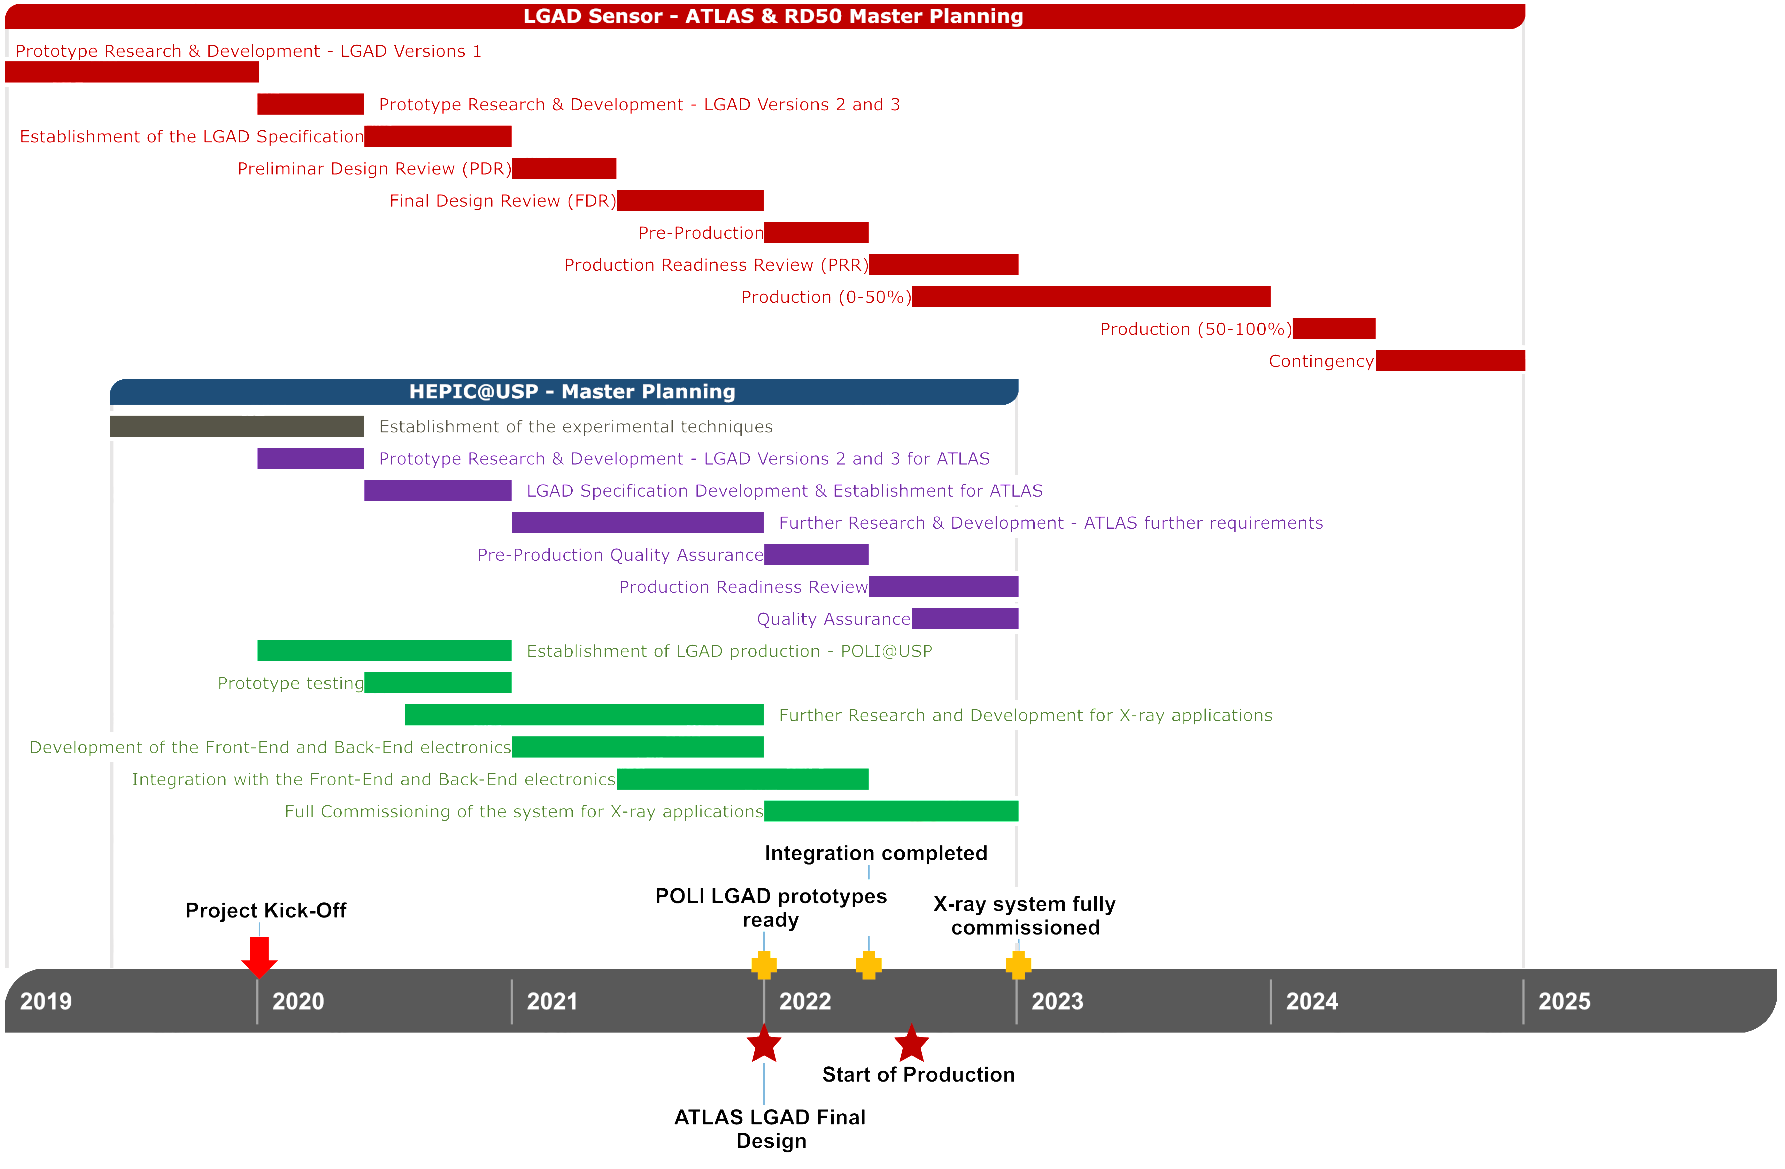
\includegraphics[width=18.0cm]{assets/cronograma.png}
    \caption{Gráfico mostrando o planejamento para o desenvolvimento do LGAD, incluindo as revisões do projeto (PDR, FDR, PRR), pré-produção e produção. Abaixo da barra azul temos o plano que será desenvolvido no HEPIC@USP visando o desenvolvimento do LGAD e suas aplicações. Os principais {\it milestones} do projeto são mostrados em sua linha do tempo.}
    \label{cronograma}
\end{figure}
\chapter{Disseminação e avaliação da pesquisa}

Uma vez que parte deste projeto está relacionada com aplicações à detecção de raios-X, essa proposta possui um grande potencial de inovação tecnológica e poderá dar origem a diversos sensores, ampliando os direitos de propriedade intelectual dos processos e dispositivos produzidos na USP. Além disso, o pesquisador responsável possui experiência no desenvolvimento de instrumentação para física de altas energias, adquirida através do trabalho realizado no projeto de {\it upgrade} do TPC do experimento ALICE \cite{tpcNIM}, isso somado à infraestrutura presente no laboratório do HEPIC para o desenvolvimento de instrumentação nuclear, tornará possível estabelecer e consolidar a linha de pesquisa em sensores semicondutores no Departamento de Física Nuclear do Instituto de Física da USP. Isso irá corroborar com programas experimentais em andamento no grupo relacionado com a espectroscopia e reconstrução de imagens com raios-X \cite{THGEM,NIM,xray}, ampliando a capacidade tecnológica do HEPIC com respeito à detecção de radiação ionizante. 

À vista disso, no âmbito nacional, com as ferramentas criadas será possível colaborar com os programas de instrumentação em diversos projetos de pesquisa presentes no Brasil tais como o Laboratório Nacional de Luz Síncrotron (LNLS), no que diz respeito ao desenvolvimento de sistemas de detecção. De acordo com os estudos levantados pelos pesquisadores do Sirius e descritas em seu projeto \cite{sirius}, {\it 'existe hoje no Brasil uma oportunidade excepcional para o desenvolvimento de expertise na área de detectores híbridos, visando atender às exigências das linhas de luz do Sirius. Futuramente, essa experiência poderá resultar em desenvolvimentos para as áreas médica, industrial e educacional'}. Isso está alinhado com os objetivos desta proposta.

No final do projeto, a infraestrutura estará consolidada e preparada para dar continuidade ao trabalho independente deste grupo em novas aplicações bem como na geração de novas tecnologias. Através da cooperação com o grupo LSI da Escola Politécnica da USP, será possível desenvolver e melhorar os sensores através de contribuições originais produzindo desse modo conhecimento e inovação.

Finalmente, com relação ao gerenciamento do projeto, o seu andamento será monitorado por meio de reuniões semanais e apresentação de resultados ao grupo, onde será reunida as informações necessária para ajustar a estratégia de modo a cumprir os objetivos propostos. Por fim, no decorrer do projeto pretende-se produzir artigos técnicos e científicos documentando os avanços obtidos no desenvolvimento dos sensores, aumentando o impacto internacional do grupo de pesquisa e da tecnologia desenvolvida no Brasil.

%\chapter{Outros apoios}

\begin{itemize}
	\item Listar os projetos em andamento que podem corroborar com este projeto
	\item Listar outros grupos brasileiros envolvidos neste upgrade
	\item Lista do bens que existem para trabalhar no upgrade
\end{itemize}

\begin{thebibliography}{9}

\bibitem{tdr} ATLAS collaboration, Technical Proposal: A High-Granularity Timing Detector for the ATLAS Phase-II Upgrade, CERN-LHCC-2018-023.

\bibitem{JIN_LGAD} N. Moffat. et al. JINST. 13, (2018) C03014.

\bibitem{NIMA_LGAD} M. Carulla. et al. Nucl. Instrum. Meth. A 924, (2019) 373. 

\bibitem{ALICEUP} ALICE Collaboration, J. Phys. G: Nucl. Part. Phys. 41 (2014) 087001.

\bibitem{ref1} B. A. et al. (ALICE Collaboration), Technical design report for the upgrade of the alice time projection chamber, CERN-LHCC-2013-020
A886 (2013), http://cds.cern.ch/record/1622286.


\bibitem{tpcNIM} M.M. Aggarwal, et al., Nucl. Instrum. Meth. A 903, (2018) 215–223. 

\bibitem{discharge_paper} A. Deisting, et al., Nucl. Instrum. Meth. A 937, (2019) 168–180.

\bibitem{COMSOL} https://www.comsol.com/comsol-multiphysics

\bibitem{THGEM} H. Natal da Luz, et al., EPJ Web of Conferences 174, (2018) 01012.

\bibitem{NIM} G. G. A. de Souza and  H. Natal da Luz, Nucl. Inst. Meth. A 937, (2019) 141–147.

\bibitem{xray} G.G.A. de Souza and H.N. da Luz, X-Ray Spectrometry 48, 5 (2018).

\bibitem{sirius} https://www.lnls.cnpem.br/sirius/livro-projeto-sirius/

%\bibitem{production_protocol} http://indico.cern.ch/event/645829/


\end{thebibliography}


\end{document}
